% MethodsX method article: RePV (Reanalysis-driven Photovoltaic Yield model).
% Headings follow the MethodsX methods article template v7 (Sept 2024). Do not rename them.
% PDF build only (build.sh). Backup of the pre-RePV version: backup_pre_repv/.
\documentclass[11pt]{article}
\usepackage[a4paper,margin=25mm]{geometry}
\usepackage[T1]{fontenc}
\usepackage{lmodern}
\usepackage{microtype}
\usepackage[british]{babel}
\usepackage{amsmath,amssymb}
\usepackage{array,booktabs,tabularx,multirow,makecell}
\usepackage{graphicx}
\usepackage{xcolor}
\usepackage{enumitem}
\usepackage{tikz}
\usetikzlibrary{positioning,arrows.meta,fit,backgrounds,calc}
\usepackage[numbers,sort&compress]{natbib}
\usepackage{xr-hyper}
\usepackage[hidelinks]{hyperref}

% Shared by main.tex and supplement.tex.
\newcommand{\todo}[1]{\textcolor{red}{[TODO: #1]}}
\newcommand{\RePV}{RePV}            % method name
% Coverage symbols of the tool comparison table (main.tex): full, partial, absent. Needs tikz where typeset.
\DeclareRobustCommand{\cF}{\tikz[baseline=-0.6ex]\fill (0,0) circle (0.55ex);}
\DeclareRobustCommand{\cH}{\tikz[baseline=-0.6ex]{\draw[line width=0.4pt] (0,0) circle (0.55ex); \fill (0,0) -- (90:0.55ex) arc (90:270:0.55ex) -- cycle;}}
\DeclareRobustCommand{\cN}{\tikz[baseline=-0.6ex]\draw[line width=0.4pt] (0,0) circle (0.55ex);}
% Validation numbers for the MethodsX manuscript. Every number in the text is a macro defined here.
%
% STATUS: PROVISIONAL. Values below come from the earlier assessment protocol
% (all hours with a value, lag fitted against clear-sky POA, no outage-day removal):
%   Lite, Core, PVGIS : per-site table of the earlier assessment (13 sites, Nevada 1367 excluded)
%   Plus              : outputs/thesis_vs_current/metrics.csv (same protocol, no bootstrap)
% Before submission, rerun all four series with the protocol of Section "Assessment design"
% (solarmodel.bench scoring + paired circular block bootstrap + PVGIS series) and regenerate this file.
% Plus has no bootstrap intervals yet; the counts marked (*) are point comparisons, not interval-based.

\newcommand{\nSites}{13}
\newcommand{\nSitesAll}{14}
\newcommand{\nBoot}{2000}
\newcommand{\blockDays}{5}

% medians across sites: bias (%), absolute bias (%), NRMSE (%), KGE, sites within +-5 %
\newcommand{\liteBias}{11.8}   \newcommand{\liteAbsBias}{11.8}  \newcommand{\liteNrmse}{71} \newcommand{\liteKge}{0.80} \newcommand{\liteWithinFive}{4}
\newcommand{\coreBias}{0.8}    \newcommand{\coreAbsBias}{12.4}  \newcommand{\coreNrmse}{74} \newcommand{\coreKge}{0.80} \newcommand{\coreWithinFive}{5}
\newcommand{\plusBias}{$-$1.0} \newcommand{\plusAbsBias}{9.9}   \newcommand{\plusNrmse}{73} \newcommand{\plusKge}{0.79} \newcommand{\plusWithinFive}{4}
\newcommand{\pvgisBias}{12.2}  \newcommand{\pvgisAbsBias}{14.4} \newcommand{\pvgisNrmse}{75} \newcommand{\pvgisKge}{0.77} \newcommand{\pvgisWithinFive}{4}

% benchmark: tier against PVGIS (median reduction in |bias| and NRMSE, percentage points; site counts)
\newcommand{\liteGainBias}{0.1}  \newcommand{\liteGainNrmse}{5.9} \newcommand{\liteCloserNrmse}{7}
\newcommand{\coreGainBias}{1.3}  \newcommand{\coreGainNrmse}{6.2} \newcommand{\coreCloserNrmse}{7}
\newcommand{\plusGainBias}{0.2}  \newcommand{\plusGainNrmse}{7.2} \newcommand{\plusCloserNrmse}{8}  % (*)
\newcommand{\coreCloserBias}{4}  \newcommand{\pvgisCloserBiasCore}{2}  % interval-based

% Plus against Core (*)
\newcommand{\plusCoreDeltaBias}{$-$1.9}
\newcommand{\plusCoreDeltaNrmse}{$-$0.3}
\newcommand{\plusCoreSmallerAbsBias}{6}
\newcommand{\plusCoreLowerNrmse}{9}

% Las Vegas single-site studies (solarmodel.bench protocol, studies/LasVegas_34)
\newcommand{\lvFixHours}{3{,}949}
\newcommand{\lvCoreBias}{+0.2}       \newcommand{\lvCoreNrmse}{21.0}
\newcommand{\lvPlusBias}{$-$1.2}     \newcommand{\lvPlusNrmse}{20.9}
\newcommand{\lvIamDelta}{$-$1.1}     \newcommand{\lvPressureDelta}{$-$0.3}
\newcommand{\lvSrcHours}{10{,}010}
\newcommand{\lvSrcCoreEraBias}{+4.2}  \newcommand{\lvSrcCoreEraNrmse}{18.0}
\newcommand{\lvSrcCoreNsrdbBias}{+0.6}\newcommand{\lvSrcCoreNsrdbNrmse}{14.6}
\newcommand{\lvSrcCoreMidcBias}{+1.9} \newcommand{\lvSrcCoreMidcNrmse}{14.5}
\newcommand{\lvSrcPlusEraBias}{+2.9}  \newcommand{\lvSrcPlusEraNrmse}{17.7}
\newcommand{\lvSrcPlusNsrdbBias}{$-$1.0}\newcommand{\lvSrcPlusNsrdbNrmse}{14.8}
\newcommand{\lvSrcPlusMidcBias}{+0.3} \newcommand{\lvSrcPlusMidcNrmse}{14.4}
\newcommand{\lvSandiaMidcBias}{+0.6}  \newcommand{\lvSandiaMidcNrmse}{14.4}
\newcommand{\lvInHours}{11{,}303}
\newcommand{\lvMosNrmseCut}{1.4}

% verification
\newcommand{\fitResidual}{$10^{-8}$}

% ---- Evidence classes (provisional; final classification depends on the provenance of U_c, U_v)
% A: metadata geometry and installed module          -> Las Vegas
% B: metadata geometry, surrogate module             -> Arbuckle, Golden, Henderson, Social Circle (assessment restricted to PVDAQ; Lausanne dropped)
% C: geometry inferred from measured output          -> Clayton 25, Clayton 27, Braga
% D: tracker or unrecorded/assumed tilt modelled as fixed -> Boulder, Cary SF1, Cary SF2, Calgary
\newcommand{\nClassA}{1} \newcommand{\nClassB}{4} \newcommand{\nClassC}{3} \newcommand{\nClassD}{4}
\newcommand{\nPrimary}{5}
% medians over the primary set (classes A and B, 6 sites): bias, |bias|, NRMSE, KGE
\newcommand{\liteBiasP}{13.1}  \newcommand{\liteAbsBiasP}{13.1}  \newcommand{\liteNrmseP}{51} \newcommand{\liteKgeP}{0.84}
\newcommand{\coreBiasP}{1.9}   \newcommand{\coreAbsBiasP}{1.9}   \newcommand{\coreNrmseP}{48} \newcommand{\coreKgeP}{0.93}
\newcommand{\plusBiasP}{0.3}   \newcommand{\plusAbsBiasP}{1.4}   \newcommand{\plusNrmseP}{48} \newcommand{\plusKgeP}{0.93}
\newcommand{\pvgisBiasP}{13.6} \newcommand{\pvgisAbsBiasP}{13.6} \newcommand{\pvgisNrmseP}{59} \newcommand{\pvgisKgeP}{0.82}
        % verification constants (\fitResidual)
% generated by make_validation_tables.py; do not edit
% Every assessment number quoted in main.tex and supplement.tex.
% Sites: 29 (Albuquerque_1429, Arbuckle_2107, CherryHill_1201, CherryHill_1202, Chester_1204, Cocoa_1403, Gaithersburg_4902, Gaithersburg_4903, Golden_10, Golden_1208, Golden_1283, Golden_1289, Golden_1432, Golden_1433, Golden_33, Golden_4, Golden_50, Golden_51, Henderson_1423, HuntValley_1199, LasVegas_1276, LasVegas_1277, LasVegas_1418, LasVegas_1420, LasVegas_34, Linthicum_1200, PresqueIsle_1239, Williston_1422, Wilmington_1203).
\newcommand{\vNScreened}{158}   % PVDAQ systems screened
\newcommand{\vNCandidates}{35}   % candidates after the metadata screen
\newcommand{\vNExcludedLate}{6}   % candidates not configured or excluded after extraction
\newcommand{\vNConfigured}{29}   % assessment sites (configured, not excluded)
\newcommand{\vNSites}{29}   % assessment sites with outputs
\newcommand{\vNInd}{25}   % independent validation sites
\newcommand{\vNCal}{4}   % calibrated sites
\newcommand{\vNClassA}{20}
\newcommand{\vNClassB}{5}
\newcommand{\vNStation}{16}   % independent sites with station irradiance
\newcommand{\vNStationAll}{16}
\newcommand{\vNStationGolden}{10}
\newcommand{\vNStationLV}{6}
\newcommand{\vNHours}{107{,}601}   % scored hours, all sites
\newcommand{\vHoursMin}{3{,}378}
\newcommand{\vHoursMax}{3{,}980}
\newcommand{\vDcMin}{1.0}
\newcommand{\vDcMax}{893}
\newcommand{\vYearMin}{2011}
\newcommand{\vYearMax}{2022}
\newcommand{\vAltMax}{1{,}995}
\newcommand{\vDegMin}{0.895}
\newcommand{\vDegMax}{0.998}
\newcommand{\vNSdm}{2}
\newcommand{\vReps}{2{,}000}
\newcommand{\vBlock}{5}
\newcommand{\vSeed}{20261109}
\newcommand{\vMedRatEraBias}{+15.3}
\newcommand{\vMedRatEraAbsBias}{15.3}
\newcommand{\vMedRatEraNrmse}{38.6}
\newcommand{\vMedRatEraKge}{0.79}
\newcommand{\vFiveRatEra}{3}
\newcommand{\vTenRatEra}{6}
\newcommand{\vMedRatNsrdbBias}{+12.3}
\newcommand{\vMedRatNsrdbAbsBias}{12.3}
\newcommand{\vMedRatNsrdbNrmse}{29.2}
\newcommand{\vMedRatNsrdbKge}{0.84}
\newcommand{\vFiveRatNsrdb}{5}
\newcommand{\vTenRatNsrdb}{11}
\newcommand{\vMedModEraBias}{+9.7}
\newcommand{\vMedModEraAbsBias}{9.7}
\newcommand{\vMedModEraNrmse}{37.5}
\newcommand{\vMedModEraKge}{0.83}
\newcommand{\vFiveModEra}{8}
\newcommand{\vTenModEra}{13}
\newcommand{\vMedModNsrdbBias}{+8.1}
\newcommand{\vMedModNsrdbAbsBias}{8.1}
\newcommand{\vMedModNsrdbNrmse}{27.5}
\newcommand{\vMedModNsrdbKge}{0.86}
\newcommand{\vFiveModNsrdb}{9}
\newcommand{\vTenModNsrdb}{14}
\newcommand{\vMedSysEraBias}{+6.7}
\newcommand{\vMedSysEraAbsBias}{6.7}
\newcommand{\vMedSysEraNrmse}{37.4}
\newcommand{\vMedSysEraKge}{0.84}
\newcommand{\vFiveSysEra}{12}
\newcommand{\vTenSysEra}{16}
\newcommand{\vMedSysNsrdbBias}{+2.6}
\newcommand{\vMedSysNsrdbAbsBias}{6.0}
\newcommand{\vMedSysNsrdbNrmse}{27.5}
\newcommand{\vMedSysNsrdbKge}{0.87}
\newcommand{\vFiveSysNsrdb}{10}
\newcommand{\vTenSysNsrdb}{18}
\newcommand{\vMedPvgisBias}{+6.5}
\newcommand{\vMedPvgisAbsBias}{6.5}
\newcommand{\vMedPvgisNrmse}{38.2}
\newcommand{\vMedPvgisKge}{0.82}
\newcommand{\vFivePvgis}{11}
\newcommand{\vTenPvgis}{15}
\newcommand{\vNPvgis}{25}
\newcommand{\vCalSysEraBias}{+4.6}
\newcommand{\vCalSysEraAbsBias}{4.6}
\newcommand{\vCalSysEraNrmse}{35.1}
\newcommand{\vCalSysEraKge}{0.85}
\newcommand{\vCalSysNsrdbBias}{+7.0}
\newcommand{\vCalSysNsrdbAbsBias}{7.0}
\newcommand{\vCalSysNsrdbNrmse}{24.9}
\newcommand{\vCalSysNsrdbKge}{0.90}
\newcommand{\vCalPvgisBias}{+2.6}
\newcommand{\vCalPvgisAbsBias}{4.3}
\newcommand{\vCalPvgisNrmse}{36.2}
\newcommand{\vCalPvgisKge}{0.85}
\newcommand{\vCalRatNsrdbBias}{+13.8}
\newcommand{\vCalRatNsrdbAbsBias}{13.8}
\newcommand{\vCalRatNsrdbNrmse}{28.1}
\newcommand{\vCalRatNsrdbKge}{0.84}
\newcommand{\vCalModNsrdbBias}{+9.5}
\newcommand{\vCalModNsrdbAbsBias}{9.5}
\newcommand{\vCalModNsrdbNrmse}{25.7}
\newcommand{\vCalModNsrdbKge}{0.88}
\newcommand{\vStnSysEraBias}{+11.0}
\newcommand{\vStnSysEraAbsBias}{11.0}
\newcommand{\vStnSysEraNrmse}{39.5}
\newcommand{\vStnSysEraKge}{0.79}
\newcommand{\vStnSysNsrdbBias}{+0.9}
\newcommand{\vStnSysNsrdbAbsBias}{5.3}
\newcommand{\vStnSysNsrdbNrmse}{30.0}
\newcommand{\vStnSysNsrdbKge}{0.86}
\newcommand{\vStnSysStnBias}{$-$0.5}
\newcommand{\vStnSysStnAbsBias}{3.8}
\newcommand{\vStnSysStnNrmse}{22.0}
\newcommand{\vStnSysStnKge}{0.89}
\newcommand{\vStnPvgisBias}{+12.6}
\newcommand{\vStnPvgisAbsBias}{12.6}
\newcommand{\vStnPvgisNrmse}{40.3}
\newcommand{\vStnPvgisKge}{0.75}
\newcommand{\vStnRatNsrdbBias}{+10.1}
\newcommand{\vStnRatNsrdbAbsBias}{10.1}
\newcommand{\vStnRatNsrdbNrmse}{31.3}
\newcommand{\vStnRatNsrdbKge}{0.84}
\newcommand{\vStnModNsrdbBias}{+4.4}
\newcommand{\vStnModNsrdbAbsBias}{5.4}
\newcommand{\vStnModNsrdbNrmse}{30.3}
\newcommand{\vStnModNsrdbKge}{0.86}
\newcommand{\vPairRatModEraAbsBetter}{20}
\newcommand{\vPairRatModEraAbsWorse}{2}
\newcommand{\vPairRatModEraAbsTie}{3}
\newcommand{\vPairRatModEraAbsMed}{+4.8}
\newcommand{\vPairRatModEraNrmseBetter}{14}
\newcommand{\vPairRatModEraNrmseWorse}{3}
\newcommand{\vPairRatModEraNrmseTie}{8}
\newcommand{\vPairRatModEraNrmseMed}{+1.0}
\newcommand{\vPairRatModEraKgeBetter}{22}
\newcommand{\vPairRatModEraKgeWorse}{1}
\newcommand{\vPairRatModEraKgeTie}{2}
\newcommand{\vPairRatModEraKgeMed}{+0.03}
\newcommand{\vPairRatModEraN}{25}
\newcommand{\vPairModSysEraAbsBetter}{18}
\newcommand{\vPairModSysEraAbsWorse}{1}
\newcommand{\vPairModSysEraAbsTie}{6}
\newcommand{\vPairModSysEraAbsMed}{+2.9}
\newcommand{\vPairModSysEraNrmseBetter}{11}
\newcommand{\vPairModSysEraNrmseWorse}{2}
\newcommand{\vPairModSysEraNrmseTie}{12}
\newcommand{\vPairModSysEraNrmseMed}{+0.9}
\newcommand{\vPairModSysEraKgeBetter}{15}
\newcommand{\vPairModSysEraKgeWorse}{4}
\newcommand{\vPairModSysEraKgeTie}{6}
\newcommand{\vPairModSysEraKgeMed}{+0.02}
\newcommand{\vPairModSysEraN}{25}
\newcommand{\vPairRatModNsrdbAbsBetter}{17}
\newcommand{\vPairRatModNsrdbAbsWorse}{2}
\newcommand{\vPairRatModNsrdbAbsTie}{6}
\newcommand{\vPairRatModNsrdbAbsMed}{+2.9}
\newcommand{\vPairRatModNsrdbNrmseBetter}{11}
\newcommand{\vPairRatModNsrdbNrmseWorse}{4}
\newcommand{\vPairRatModNsrdbNrmseTie}{10}
\newcommand{\vPairRatModNsrdbNrmseMed}{+0.7}
\newcommand{\vPairRatModNsrdbKgeBetter}{18}
\newcommand{\vPairRatModNsrdbKgeWorse}{1}
\newcommand{\vPairRatModNsrdbKgeTie}{6}
\newcommand{\vPairRatModNsrdbKgeMed}{+0.02}
\newcommand{\vPairRatModNsrdbN}{25}
\newcommand{\vPairModSysNsrdbAbsBetter}{14}
\newcommand{\vPairModSysNsrdbAbsWorse}{4}
\newcommand{\vPairModSysNsrdbAbsTie}{7}
\newcommand{\vPairModSysNsrdbAbsMed}{+1.9}
\newcommand{\vPairModSysNsrdbNrmseBetter}{7}
\newcommand{\vPairModSysNsrdbNrmseWorse}{4}
\newcommand{\vPairModSysNsrdbNrmseTie}{14}
\newcommand{\vPairModSysNsrdbNrmseMed}{+0.2}
\newcommand{\vPairModSysNsrdbKgeBetter}{13}
\newcommand{\vPairModSysNsrdbKgeWorse}{4}
\newcommand{\vPairModSysNsrdbKgeTie}{8}
\newcommand{\vPairModSysNsrdbKgeMed}{+0.01}
\newcommand{\vPairModSysNsrdbN}{25}
\newcommand{\vPairRatModStnAbsBetter}{11}
\newcommand{\vPairRatModStnAbsWorse}{0}
\newcommand{\vPairRatModStnAbsTie}{5}
\newcommand{\vPairRatModStnAbsMed}{+2.8}
\newcommand{\vPairRatModStnNrmseBetter}{8}
\newcommand{\vPairRatModStnNrmseWorse}{3}
\newcommand{\vPairRatModStnNrmseTie}{5}
\newcommand{\vPairRatModStnNrmseMed}{+1.1}
\newcommand{\vPairRatModStnKgeBetter}{9}
\newcommand{\vPairRatModStnKgeWorse}{1}
\newcommand{\vPairRatModStnKgeTie}{6}
\newcommand{\vPairRatModStnKgeMed}{+0.01}
\newcommand{\vPairRatModStnN}{16}
\newcommand{\vPairModSysStnAbsBetter}{8}
\newcommand{\vPairModSysStnAbsWorse}{4}
\newcommand{\vPairModSysStnAbsTie}{4}
\newcommand{\vPairModSysStnAbsMed}{+1.9}
\newcommand{\vPairModSysStnNrmseBetter}{4}
\newcommand{\vPairModSysStnNrmseWorse}{3}
\newcommand{\vPairModSysStnNrmseTie}{9}
\newcommand{\vPairModSysStnNrmseMed}{+0.1}
\newcommand{\vPairModSysStnKgeBetter}{7}
\newcommand{\vPairModSysStnKgeWorse}{4}
\newcommand{\vPairModSysStnKgeTie}{5}
\newcommand{\vPairModSysStnKgeMed}{+0.01}
\newcommand{\vPairModSysStnN}{16}
\newcommand{\vPairEraNsrdbAbsBetter}{10}
\newcommand{\vPairEraNsrdbAbsWorse}{7}
\newcommand{\vPairEraNsrdbAbsTie}{8}
\newcommand{\vPairEraNsrdbAbsMed}{+0.8}
\newcommand{\vPairEraNsrdbNrmseBetter}{25}
\newcommand{\vPairEraNsrdbNrmseWorse}{0}
\newcommand{\vPairEraNsrdbNrmseTie}{0}
\newcommand{\vPairEraNsrdbNrmseMed}{+7.8}
\newcommand{\vPairEraNsrdbKgeBetter}{21}
\newcommand{\vPairEraNsrdbKgeWorse}{0}
\newcommand{\vPairEraNsrdbKgeTie}{4}
\newcommand{\vPairEraNsrdbKgeMed}{+0.05}
\newcommand{\vPairEraNsrdbN}{25}
\newcommand{\vPairNsrdbStnAbsBetter}{5}
\newcommand{\vPairNsrdbStnAbsWorse}{3}
\newcommand{\vPairNsrdbStnAbsTie}{8}
\newcommand{\vPairNsrdbStnAbsMed}{+0.4}
\newcommand{\vPairNsrdbStnNrmseBetter}{10}
\newcommand{\vPairNsrdbStnNrmseWorse}{2}
\newcommand{\vPairNsrdbStnNrmseTie}{4}
\newcommand{\vPairNsrdbStnNrmseMed}{+2.5}
\newcommand{\vPairNsrdbStnKgeBetter}{11}
\newcommand{\vPairNsrdbStnKgeWorse}{1}
\newcommand{\vPairNsrdbStnKgeTie}{4}
\newcommand{\vPairNsrdbStnKgeMed}{+0.01}
\newcommand{\vPairNsrdbStnN}{16}
\newcommand{\vPairEraPvgisAbsBetter}{5}
\newcommand{\vPairEraPvgisAbsWorse}{9}
\newcommand{\vPairEraPvgisAbsTie}{11}
\newcommand{\vPairEraPvgisAbsMed}{$-$0.5}
\newcommand{\vPairEraPvgisNrmseBetter}{8}
\newcommand{\vPairEraPvgisNrmseWorse}{6}
\newcommand{\vPairEraPvgisNrmseTie}{11}
\newcommand{\vPairEraPvgisNrmseMed}{$-$0.3}
\newcommand{\vPairEraPvgisKgeBetter}{9}
\newcommand{\vPairEraPvgisKgeWorse}{9}
\newcommand{\vPairEraPvgisKgeTie}{7}
\newcommand{\vPairEraPvgisKgeMed}{0.00}
\newcommand{\vPairEraPvgisN}{25}
\newcommand{\vPairPvgisNsrdbAbsBetter}{10}
\newcommand{\vPairPvgisNsrdbAbsWorse}{6}
\newcommand{\vPairPvgisNsrdbAbsTie}{9}
\newcommand{\vPairPvgisNsrdbAbsMed}{+0.3}
\newcommand{\vPairPvgisNsrdbNrmseBetter}{21}
\newcommand{\vPairPvgisNsrdbNrmseWorse}{0}
\newcommand{\vPairPvgisNsrdbNrmseTie}{4}
\newcommand{\vPairPvgisNsrdbNrmseMed}{+7.7}
\newcommand{\vPairPvgisNsrdbKgeBetter}{17}
\newcommand{\vPairPvgisNsrdbKgeWorse}{4}
\newcommand{\vPairPvgisNsrdbKgeTie}{4}
\newcommand{\vPairPvgisNsrdbKgeMed}{+0.06}
\newcommand{\vPairPvgisNsrdbN}{25}
\newcommand{\vStepZeroEraBias}{$-$4.83}
\newcommand{\vStepZeroEraNrmse}{$-$1.02}
\newcommand{\vStepZeroEraMin}{$-$14.2}
\newcommand{\vStepZeroEraMax}{+1.0}
\newcommand{\vStepZeroEraAct}{25}
\newcommand{\vStepZeroNsrdbBias}{$-$4.50}
\newcommand{\vStepZeroNsrdbNrmse}{$-$0.67}
\newcommand{\vStepZeroNsrdbMin}{$-$14.1}
\newcommand{\vStepZeroNsrdbMax}{+1.6}
\newcommand{\vStepZeroNsrdbAct}{25}
\newcommand{\vStepOneEraBias}{$-$0.32}
\newcommand{\vStepOneEraNrmse}{$-$0.02}
\newcommand{\vStepOneEraMin}{$-$1.0}
\newcommand{\vStepOneEraMax}{0.0}
\newcommand{\vStepOneEraAct}{18}
\newcommand{\vStepOneNsrdbBias}{$-$0.31}
\newcommand{\vStepOneNsrdbNrmse}{$-$0.01}
\newcommand{\vStepOneNsrdbMin}{$-$0.9}
\newcommand{\vStepOneNsrdbMax}{0.0}
\newcommand{\vStepOneNsrdbAct}{18}
\newcommand{\vStepTwoEraBias}{$-$1.55}
\newcommand{\vStepTwoEraNrmse}{$-$0.54}
\newcommand{\vStepTwoEraMin}{$-$2.1}
\newcommand{\vStepTwoEraMax}{$-$1.0}
\newcommand{\vStepTwoEraAct}{25}
\newcommand{\vStepTwoNsrdbBias}{$-$1.70}
\newcommand{\vStepTwoNsrdbNrmse}{$-$0.26}
\newcommand{\vStepTwoNsrdbMin}{$-$2.5}
\newcommand{\vStepTwoNsrdbMax}{$-$1.0}
\newcommand{\vStepTwoNsrdbAct}{25}
\newcommand{\vStepThreeEraBias}{0.00}
\newcommand{\vStepThreeEraNrmse}{0.00}
\newcommand{\vStepThreeEraMin}{0.0}
\newcommand{\vStepThreeEraMax}{0.0}
\newcommand{\vStepThreeEraAct}{0}
\newcommand{\vStepThreeNsrdbBias}{0.00}
\newcommand{\vStepThreeNsrdbNrmse}{0.00}
\newcommand{\vStepThreeNsrdbMin}{0.0}
\newcommand{\vStepThreeNsrdbMax}{0.0}
\newcommand{\vStepThreeNsrdbAct}{0}
\newcommand{\vStepFourEraBias}{$-$0.01}
\newcommand{\vStepFourEraNrmse}{0.00}
\newcommand{\vStepFourEraMin}{$-$0.3}
\newcommand{\vStepFourEraMax}{+0.4}
\newcommand{\vStepFourEraAct}{6}
\newcommand{\vStepFourNsrdbBias}{$-$0.01}
\newcommand{\vStepFourNsrdbNrmse}{0.00}
\newcommand{\vStepFourNsrdbMin}{$-$0.4}
\newcommand{\vStepFourNsrdbMax}{+0.3}
\newcommand{\vStepFourNsrdbAct}{4}
\newcommand{\vStepFiveEraBias}{0.00}
\newcommand{\vStepFiveEraNrmse}{0.00}
\newcommand{\vStepFiveEraMin}{$-$0.2}
\newcommand{\vStepFiveEraMax}{+0.2}
\newcommand{\vStepFiveEraAct}{4}
\newcommand{\vStepFiveNsrdbBias}{0.00}
\newcommand{\vStepFiveNsrdbNrmse}{0.00}
\newcommand{\vStepFiveNsrdbMin}{$-$0.2}
\newcommand{\vStepFiveNsrdbMax}{+0.3}
\newcommand{\vStepFiveNsrdbAct}{3}
\newcommand{\vStepSixEraBias}{0.00}
\newcommand{\vStepSixEraNrmse}{0.00}
\newcommand{\vStepSixEraMin}{$-$0.2}
\newcommand{\vStepSixEraMax}{0.0}
\newcommand{\vStepSixEraAct}{1}
\newcommand{\vStepSixNsrdbBias}{0.00}
\newcommand{\vStepSixNsrdbNrmse}{0.00}
\newcommand{\vStepSixNsrdbMin}{$-$0.1}
\newcommand{\vStepSixNsrdbMax}{0.0}
\newcommand{\vStepSixNsrdbAct}{1}
\newcommand{\vStepSevenEraBias}{0.00}
\newcommand{\vStepSevenEraNrmse}{0.00}
\newcommand{\vStepSevenEraMin}{0.0}
\newcommand{\vStepSevenEraMax}{0.0}
\newcommand{\vStepSevenEraAct}{0}
\newcommand{\vStepSevenNsrdbBias}{0.00}
\newcommand{\vStepSevenNsrdbNrmse}{0.00}
\newcommand{\vStepSevenNsrdbMin}{0.0}
\newcommand{\vStepSevenNsrdbMax}{0.0}
\newcommand{\vStepSevenNsrdbAct}{0}
\newcommand{\vStepEightEraBias}{$-$1.75}
\newcommand{\vStepEightEraNrmse}{$-$0.12}
\newcommand{\vStepEightEraMin}{$-$7.6}
\newcommand{\vStepEightEraMax}{0.0}
\newcommand{\vStepEightEraAct}{17}
\newcommand{\vStepEightNsrdbBias}{$-$1.39}
\newcommand{\vStepEightNsrdbNrmse}{0.00}
\newcommand{\vStepEightNsrdbMin}{$-$6.0}
\newcommand{\vStepEightNsrdbMax}{0.0}
\newcommand{\vStepEightNsrdbAct}{17}
\newcommand{\vStepNineEraBias}{+0.03}
\newcommand{\vStepNineEraNrmse}{+0.01}
\newcommand{\vStepNineEraMin}{0.0}
\newcommand{\vStepNineEraMax}{+1.5}
\newcommand{\vStepNineEraAct}{8}
\newcommand{\vStepNineNsrdbBias}{+0.02}
\newcommand{\vStepNineNsrdbNrmse}{0.00}
\newcommand{\vStepNineNsrdbMin}{0.0}
\newcommand{\vStepNineNsrdbMax}{+1.4}
\newcommand{\vStepNineNsrdbAct}{8}
\newcommand{\vStepTenEraBias}{0.00}
\newcommand{\vStepTenEraNrmse}{0.00}
\newcommand{\vStepTenEraMin}{0.0}
\newcommand{\vStepTenEraMax}{0.0}
\newcommand{\vStepTenEraAct}{0}
\newcommand{\vStepTenNsrdbBias}{0.00}
\newcommand{\vStepTenNsrdbNrmse}{0.00}
\newcommand{\vStepTenNsrdbMin}{0.0}
\newcommand{\vStepTenNsrdbMax}{0.0}
\newcommand{\vStepTenNsrdbAct}{0}
\newcommand{\vStepSdmEraBias}{$-$0.37}
\newcommand{\vStepSdmEraNrmse}{$-$0.38}
\newcommand{\vStepSdmEraMin}{$-$1.0}
\newcommand{\vStepSdmEraMax}{+0.2}
\newcommand{\vStepSdmEraAct}{2}
\newcommand{\vStepSdmNsrdbBias}{$-$0.50}
\newcommand{\vStepSdmNsrdbNrmse}{$-$0.57}
\newcommand{\vStepSdmNsrdbMin}{$-$1.2}
\newcommand{\vStepSdmNsrdbMax}{+0.2}
\newcommand{\vStepSdmNsrdbAct}{2}
\newcommand{\vSysNsrdbBiasLo}{$-$11.7}
\newcommand{\vSysNsrdbBiasHi}{+13.6}
\newcommand{\vPathRatNrmseGainEra}{2.3}
\newcommand{\vPathModNrmseGainEra}{0.9}
\newcommand{\vInputNrmseGain}{7.8}
\newcommand{\vInputNrmseGainLo}{1.2}
\newcommand{\vInputNrmseGainHi}{21.4}
\newcommand{\vNInputBeatsPath}{22}
\newcommand{\vNGolden}{10}
\newcommand{\vGoldenEraBiasLo}{$-$1.6}
\newcommand{\vGoldenEraBiasHi}{+27.2}
\newcommand{\vGoldenEraBiasMed}{+20.1}
\newcommand{\vGoldenNsrdbBiasLo}{$-$11.7}
\newcommand{\vGoldenNsrdbBiasHi}{+12.1}
\newcommand{\vGoldenNsrdbBiasMed}{+5.8}
\newcommand{\vGoldenStnBiasLo}{$-$11.1}
\newcommand{\vGoldenStnBiasHi}{+13.7}
\newcommand{\vGoldenStnBiasMed}{+5.0}
\newcommand{\vGoldenPvgisBiasLo}{$-$2.5}
\newcommand{\vGoldenPvgisBiasHi}{+36.3}
\newcommand{\vNDesert}{6}
\newcommand{\vDesertEraBiasLo}{$-$4.1}
\newcommand{\vDesertEraBiasHi}{+3.7}
\newcommand{\vDesertEraBiasMed}{$-$0.3}
\newcommand{\vDesertNsrdbBiasLo}{$-$6.7}
\newcommand{\vDesertNsrdbBiasHi}{+2.6}
\newcommand{\vDesertNsrdbBiasMed}{$-$1.6}
\newcommand{\vDesertStnBiasLo}{$-$6.3}
\newcommand{\vDesertStnBiasHi}{+1.1}
\newcommand{\vDesertStnBiasMed}{$-$2.3}
\newcommand{\vDesertPvgisBiasLo}{$-$1.1}
\newcommand{\vDesertPvgisBiasHi}{+4.5}
\newcommand{\vNEast}{7}
\newcommand{\vEastEraBiasLo}{$-$3.9}
\newcommand{\vEastEraBiasHi}{+16.7}
\newcommand{\vEastEraBiasMed}{+3.4}
\newcommand{\vEastNsrdbBiasLo}{$-$3.1}
\newcommand{\vEastNsrdbBiasHi}{+13.6}
\newcommand{\vEastNsrdbBiasMed}{+8.4}
\newcommand{\vEastPvgisBiasLo}{$-$3.6}
\newcommand{\vEastPvgisBiasHi}{+13.3}
\newcommand{\vHorizonMax}{9.9}
\newcommand{\vNHorizon}{29}
\newcommand{\vPvgisBeatsSysEraNrmse}{11}
\newcommand{\vNsrdbBeatsPvgisNrmse}{25}
\newcommand{\vNsrdbBeatsEraNrmse}{25}
\newcommand{\vAblPresModEra}{$-$0.32}
\newcommand{\vAblPresModEraLo}{$-$1.0}
\newcommand{\vAblPresModEraHi}{0.0}
\newcommand{\vAblPresModEraAct}{18}
\newcommand{\vAblPresSysEra}{$-$0.32}
\newcommand{\vAblPresSysEraLo}{$-$1.1}
\newcommand{\vAblPresSysEraHi}{0.0}
\newcommand{\vAblPresSysEraAct}{18}
\newcommand{\vAblPresModNsrdb}{$-$0.31}
\newcommand{\vAblPresModNsrdbLo}{$-$0.9}
\newcommand{\vAblPresModNsrdbHi}{0.0}
\newcommand{\vAblPresModNsrdbAct}{18}
\newcommand{\vAblPresSysNsrdb}{$-$0.31}
\newcommand{\vAblPresSysNsrdbLo}{$-$1.0}
\newcommand{\vAblPresSysNsrdbHi}{0.0}
\newcommand{\vAblPresSysNsrdbAct}{18}
\newcommand{\vAblIamModEra}{$-$1.55}
\newcommand{\vAblIamModEraLo}{$-$2.1}
\newcommand{\vAblIamModEraHi}{$-$1.0}
\newcommand{\vAblIamModEraAct}{25}
\newcommand{\vAblIamSysEra}{$-$1.69}
\newcommand{\vAblIamSysEraLo}{$-$2.1}
\newcommand{\vAblIamSysEraHi}{$-$1.0}
\newcommand{\vAblIamSysEraAct}{25}
\newcommand{\vAblIamModNsrdb}{$-$1.70}
\newcommand{\vAblIamModNsrdbLo}{$-$2.5}
\newcommand{\vAblIamModNsrdbHi}{$-$1.0}
\newcommand{\vAblIamModNsrdbAct}{25}
\newcommand{\vAblIamSysNsrdb}{$-$1.86}
\newcommand{\vAblIamSysNsrdbLo}{$-$2.4}
\newcommand{\vAblIamSysNsrdbHi}{$-$1.1}
\newcommand{\vAblIamSysNsrdbAct}{25}
\newcommand{\vAblHorModEra}{0.00}
\newcommand{\vAblHorModEraLo}{0.0}
\newcommand{\vAblHorModEraHi}{0.0}
\newcommand{\vAblHorModEraAct}{0}
\newcommand{\vAblHorSysEra}{0.00}
\newcommand{\vAblHorSysEraLo}{0.0}
\newcommand{\vAblHorSysEraHi}{0.0}
\newcommand{\vAblHorSysEraAct}{0}
\newcommand{\vAblHorModNsrdb}{0.00}
\newcommand{\vAblHorModNsrdbLo}{0.0}
\newcommand{\vAblHorModNsrdbHi}{0.0}
\newcommand{\vAblHorModNsrdbAct}{0}
\newcommand{\vAblHorSysNsrdb}{0.00}
\newcommand{\vAblHorSysNsrdbLo}{0.0}
\newcommand{\vAblHorSysNsrdbHi}{0.0}
\newcommand{\vAblHorSysNsrdbAct}{0}
\newcommand{\vAblLossModEra}{$-$0.01}
\newcommand{\vAblLossModEraLo}{$-$0.4}
\newcommand{\vAblLossModEraHi}{+0.6}
\newcommand{\vAblLossModEraAct}{9}
\newcommand{\vAblLossSysEra}{$-$0.02}
\newcommand{\vAblLossSysEraLo}{$-$0.1}
\newcommand{\vAblLossSysEraHi}{+0.4}
\newcommand{\vAblLossSysEraAct}{6}
\newcommand{\vAblLossModNsrdb}{$-$0.01}
\newcommand{\vAblLossModNsrdbLo}{$-$0.5}
\newcommand{\vAblLossModNsrdbHi}{+0.4}
\newcommand{\vAblLossModNsrdbAct}{6}
\newcommand{\vAblLossSysNsrdb}{$-$0.02}
\newcommand{\vAblLossSysNsrdbLo}{$-$0.1}
\newcommand{\vAblLossSysNsrdbHi}{+0.3}
\newcommand{\vAblLossSysNsrdbAct}{4}
\newcommand{\vAblSoilModEra}{+0.01}
\newcommand{\vAblSoilModEraLo}{$-$0.2}
\newcommand{\vAblSoilModEraHi}{+0.2}
\newcommand{\vAblSoilModEraAct}{5}
\newcommand{\vAblSoilSysEra}{0.00}
\newcommand{\vAblSoilSysEraLo}{$-$0.2}
\newcommand{\vAblSoilSysEraHi}{+0.3}
\newcommand{\vAblSoilSysEraAct}{5}
\newcommand{\vAblSoilModNsrdb}{0.00}
\newcommand{\vAblSoilModNsrdbLo}{$-$0.2}
\newcommand{\vAblSoilModNsrdbHi}{+0.2}
\newcommand{\vAblSoilModNsrdbAct}{4}
\newcommand{\vAblSoilSysNsrdb}{0.00}
\newcommand{\vAblSoilSysNsrdbLo}{$-$0.2}
\newcommand{\vAblSoilSysNsrdbHi}{+0.3}
\newcommand{\vAblSoilSysNsrdbAct}{4}
\newcommand{\vAblClipModEra}{0.00}
\newcommand{\vAblClipModEraLo}{$-$0.5}
\newcommand{\vAblClipModEraHi}{0.0}
\newcommand{\vAblClipModEraAct}{2}
\newcommand{\vAblClipSysEra}{0.00}
\newcommand{\vAblClipSysEraLo}{$-$0.2}
\newcommand{\vAblClipSysEraHi}{0.0}
\newcommand{\vAblClipSysEraAct}{1}
\newcommand{\vAblClipModNsrdb}{0.00}
\newcommand{\vAblClipModNsrdbLo}{$-$0.7}
\newcommand{\vAblClipModNsrdbHi}{0.0}
\newcommand{\vAblClipModNsrdbAct}{3}
\newcommand{\vAblClipSysNsrdb}{0.00}
\newcommand{\vAblClipSysNsrdbLo}{$-$0.1}
\newcommand{\vAblClipSysNsrdbHi}{0.0}
\newcommand{\vAblClipSysNsrdbAct}{1}
\newcommand{\vAblDepthModEra}{0.00}
\newcommand{\vAblDepthModEraLo}{0.0}
\newcommand{\vAblDepthModEraHi}{0.0}
\newcommand{\vAblDepthModEraAct}{0}
\newcommand{\vAblDepthSysEra}{0.00}
\newcommand{\vAblDepthSysEraLo}{0.0}
\newcommand{\vAblDepthSysEraHi}{0.0}
\newcommand{\vAblDepthSysEraAct}{0}
\newcommand{\vAblDepthModNsrdb}{0.00}
\newcommand{\vAblDepthModNsrdbLo}{0.0}
\newcommand{\vAblDepthModNsrdbHi}{0.0}
\newcommand{\vAblDepthModNsrdbAct}{0}
\newcommand{\vAblDepthSysNsrdb}{0.00}
\newcommand{\vAblDepthSysNsrdbLo}{0.0}
\newcommand{\vAblDepthSysNsrdbHi}{0.0}
\newcommand{\vAblDepthSysNsrdbAct}{0}
\newcommand{\vAblTrigModEra}{$-$1.76}
\newcommand{\vAblTrigModEraLo}{$-$7.8}
\newcommand{\vAblTrigModEraHi}{0.0}
\newcommand{\vAblTrigModEraAct}{17}
\newcommand{\vAblTrigSysEra}{$-$1.75}
\newcommand{\vAblTrigSysEraLo}{$-$7.6}
\newcommand{\vAblTrigSysEraHi}{0.0}
\newcommand{\vAblTrigSysEraAct}{17}
\newcommand{\vAblTrigModNsrdb}{$-$1.41}
\newcommand{\vAblTrigModNsrdbLo}{$-$6.1}
\newcommand{\vAblTrigModNsrdbHi}{0.0}
\newcommand{\vAblTrigModNsrdbAct}{17}
\newcommand{\vAblTrigSysNsrdb}{$-$1.39}
\newcommand{\vAblTrigSysNsrdbLo}{$-$6.0}
\newcommand{\vAblTrigSysNsrdbHi}{0.0}
\newcommand{\vAblTrigSysNsrdbAct}{17}
\newcommand{\vAblAlbModEra}{+0.10}
\newcommand{\vAblAlbModEraLo}{0.0}
\newcommand{\vAblAlbModEraHi}{+1.6}
\newcommand{\vAblAlbModEraAct}{12}
\newcommand{\vAblAlbSysEra}{+0.03}
\newcommand{\vAblAlbSysEraLo}{0.0}
\newcommand{\vAblAlbSysEraHi}{+1.5}
\newcommand{\vAblAlbSysEraAct}{8}
\newcommand{\vAblAlbModNsrdb}{+0.07}
\newcommand{\vAblAlbModNsrdbLo}{0.0}
\newcommand{\vAblAlbModNsrdbHi}{+1.5}
\newcommand{\vAblAlbModNsrdbAct}{10}
\newcommand{\vAblAlbSysNsrdb}{+0.02}
\newcommand{\vAblAlbSysNsrdbLo}{0.0}
\newcommand{\vAblAlbSysNsrdbHi}{+1.4}
\newcommand{\vAblAlbSysNsrdbAct}{8}
\newcommand{\vAblSnowModEra}{$-$0.11}
\newcommand{\vAblSnowModEraLo}{$-$10.0}
\newcommand{\vAblSnowModEraHi}{0.0}
\newcommand{\vAblSnowModEraAct}{13}
\newcommand{\vAblSnowSysEra}{$-$2.08}
\newcommand{\vAblSnowSysEraLo}{$-$17.5}
\newcommand{\vAblSnowSysEraHi}{0.0}
\newcommand{\vAblSnowSysEraAct}{17}
\newcommand{\vAblSnowModNsrdb}{$-$0.10}
\newcommand{\vAblSnowModNsrdbLo}{$-$10.2}
\newcommand{\vAblSnowModNsrdbHi}{0.0}
\newcommand{\vAblSnowModNsrdbAct}{13}
\newcommand{\vAblSnowSysNsrdb}{$-$2.11}
\newcommand{\vAblSnowSysNsrdbLo}{$-$15.8}
\newcommand{\vAblSnowSysNsrdbHi}{0.0}
\newcommand{\vAblSnowSysNsrdbAct}{17}
\newcommand{\vBmsDistMin}{0.3}
\newcommand{\vBmsDistMax}{1}
\newcommand{\vUnlvDistMin}{6.6}
\newcommand{\vUnlvDistMax}{22}
\newcommand{\vUcFit}{1}
\newcommand{\vUcNoct}{3}
\newcommand{\vUcClass}{25}
    % assessment numbers, written by make_validation_tables.py

\newcommand{\rot}[1]{\rotatebox{90}{\makecell[l]{#1}}}
\externaldocument{build/supplement}   % Table S*, Section S* references; build supplement.tex first (build.sh)

\begin{document}

%===========================================================================
\section*{Article information}

\paragraph{Article title}
RePV: An open, configuration-driven physical modelling pipeline for photovoltaic power estimation

\paragraph{Authors}
Priyam Ketan Bhavsar\textsuperscript{a,*}

\paragraph{Affiliations}
\textsuperscript{a}\,Technical University of Munich, School of Engineering, 80333 Munich, Germany

\paragraph{Corresponding author's email address}
priyam.bhavsar@tum.de

\paragraph{Keywords}
Photovoltaic energy yield; ERA5 reanalysis; chronological power series; snow and soiling losses; reproducible modelling; open-source modelling; pvlib; model validation

\paragraph{Related research article}
None

%===========================================================================
\section*{Abstract}

Chronological photovoltaic (PV) power series are required for prospective site assessment, storage sizing and hybrid-system simulation, but measured irradiance, operating data and complete system descriptions are rarely available at candidate sites. \RePV{} (Reanalysis-driven Photovoltaic Yield model) is an open method that converts weather data and a description of the PV system into AC power at the grid connection point, using a fixed sequence of published models. Its contribution is that every modelling decision that affects the result is fixed and documented: the order of the models, the source of each parameter value, the time interval that each value represents, the starting state of snow and soiling, the default used when an input is missing, and whether each loss acts before or after the inverter. The irradiance input can be exchanged for another source, and intermediate results are returned for checking. Two adaptations of the NREL snow model to hourly reanalysis inputs are introduced, and its published ground-snow-depth condition is driven by ERA5-Land snow depth. \RePV{} was validated against measured AC output from \vNInd{} fixed-tilt systems of the NREL PVDAQ archive, configured from metadata alone, with ERA5, NSRDB and ground-station irradiance as inputs and PVGIS as an independently developed reference model. On ERA5, the median absolute energy bias was \vMedSysEraAbsBias\,\%, against \vMedRatEraAbsBias\,\% for a simple model that scales the module rating with irradiance and temperature, and \vMedPvgisAbsBias\,\% for PVGIS. Replacing ERA5 with NSRDB irradiance lowered the hourly NRMSE by a median of \vInputNrmseGain{} points per site, and replacing the simple model with \RePV{} by \vPathRatNrmseGainEra{} points. The hour-to-hour error therefore depends mainly on the irradiance source, whereas the error in total energy depends more on how irradiance is converted into power.

\begin{itemize}
    \item A fixed, documented sequence of physical models converts open weather data into the AC power of a PV system.
    \item Each system file records the parameter values, where each value came from, the model choices and the defaults used.
    \item Validation with three irradiance sources separates errors of the weather input from errors of the conversion to power.
\end{itemize}

%===========================================================================
\section*{Specifications table}

\begin{table}[h]
\centering
\small
\begin{tabularx}{\textwidth}{>{\bfseries}p{0.30\textwidth} X}
\toprule
Subject area & Energy \\
More specific subject area & Configurable physical modelling of photovoltaic power from open meteorological data \\
Name of your method & \RePV: Reanalysis-driven Photovoltaic Yield model \\
Name and reference of original method &
De Soto single-diode model~\cite{desotoImprovementValidationModel2006};
Reindl sky-diffuse transposition~\cite{reindlEvaluationHourly1990};
PVsyst heat-balance cell-temperature model~\cite{pvsystUvalueMeasurement2026,faimanAssessingOutdoor2008};
NREL snow-coverage model~\cite{marionMeasuredPhotovoltaicSystem2013,rybergIntegrationValidationApplication2017};
Kimber soiling model~\cite{kimber2006};
PVWatts inverter model~\cite{dobosPVWattsVersion52014};
pvlib python~\cite{holmgrenPvlibPythonPython2018,anderson2023pvlib}. \\
Resource availability &
Code: \url{https://github.com/princepriyam/RePV} and archived release \href{https://doi.org/10.5281/zenodo.24355624}{doi:10.5281/zenodo.24355624}, MIT licence.
Weather: ERA5~\cite{hersbachERA5Global2020} and ERA5-Land~\cite{munozsabater2021era5land} through the Open-Meteo archive API~\cite{zippenfenig2023openmeteo}.
Horizon profile and benchmark: PVGIS API v5.3~\cite{huldNewSolarRadiation2012}.
Measured data: NREL PVDAQ~\cite{deline2021pvdaq}.
Comparison irradiance: NSRDB~\cite{sengupta2018nsrdb} and the NREL MIDC stations BMS and UNLV~\cite{andreasStoffel1981bms,andreasStoffel2006unlv}. \\
\bottomrule
\end{tabularx}
\end{table}

%===========================================================================
\section{Background}
\label{sec:background}

Capacity, storage and operating decisions for hybrid plants at prospective PV sites are assessed with chronological power series rather than annual or monthly energy totals, because the timing and persistence of PV generation govern storage operation and energy deficits. At such sites, measured output and observations of snow, soiling and other losses are unavailable, and ground irradiance measurements are often incomplete or absent. Global reanalysis supplies consistent irradiance and meteorological variables for any location and year since 1940~\cite{hersbachERA5Global2020}, at the cost of larger hourly irradiance errors than ground or satellite data~\cite{urraca2018era5}. Converting these variables into AC power requires an ordered sequence of geometric, transposition, optical, environmental, thermal, electrical and loss models.

Existing tools provide this conversion at two levels. End-to-end services such as PVGIS~\cite{huldNewSolarRadiation2012,suri2008pvgis} return chronological output from a few site and system inputs, but fix which models are used and combine the system losses into one percentage. Component libraries such as pvlib python~\cite{holmgrenPvlibPythonPython2018,anderson2023pvlib} implement individual models transparently but leave their selection, parameterisation and connection to the user. The result depends on the equations and equally on the decisions around them: the order of the models, where parameter values come from, which time interval each value represents, how snow and soiling start, and whether a loss acts before or after the inverter. Services make these decisions internally, libraries leave them to the user, and neither documents them as one complete, repeatable procedure. Table~\ref{tab:tools} lists the stages of the chain that widely used tools include in their standard calculation chain. Most stages are available somewhere in these tools; the table shows which are connected into one documented procedure, not whether a capability exists.

\begin{table}[htbp]
\centering
\caption{Stages of the PV power chain in the standard calculation chain of widely used tools and of \RePV{}, from their documentation accessed in November 2026: PVGIS~5.3, SAM~2025.4.16, PVsyst~8, atlite~0.7, the pvlib python~0.16.1 \texttt{ModelChain}, and the Renewables.ninja and HOMER Pro web documentation. \cF{}: the tool computes the stage, or retrieves its input, as part of its standard calculation chain; \cN{}: absent, represented only by fixed monthly values or one combined loss, or possible only when the user prepares the input outside the tool (for example a horizon converted to a shading table) or connects a separate function.}
\label{tab:tools}
\small
\setlength{\tabcolsep}{3.6pt}
\begin{tabular}{l *{10}{c}}
\toprule
 & \rot{Reanalysis\\weather} & \rot{Terrain\\horizon} & \rot{Row\\shading} & \rot{Incidence angle\\and spectrum} & \rot{Snow\\cover} & \rot{Rain-driven\\soiling} & \rot{Heat-balance\\cell temperature} & \rot{Single-diode\\DC model} & \rot{DC and AC\\losses separated} & \rot{Site AC\\limit} \\
\midrule
PVGIS~\cite{huldNewSolarRadiation2012,huldGraciaAmillo2015} & \cF & \cF & \cN & \cF & \cN & \cN & \cF & \cN & \cN & \cN \\
Renewables.ninja~\cite{pfenningerStaffell2016} & \cF & \cN & \cN & \cN & \cN & \cN & \cN & \cN & \cN & \cN \\
atlite~\cite{hofmann2021atlite} & \cF & \cN & \cN & \cN & \cN & \cN & \cN & \cN & \cN & \cN \\
HOMER Pro~\cite{lambert2006homer} & \cN & \cN & \cN & \cN & \cN & \cN & \cF & \cN & \cN & \cF \\
PVsyst~\cite{pvsystHelp2026} & \cN & \cF & \cF & \cF & \cN & \cN & \cF & \cF & \cF & \cF \\
SAM~\cite{gilmanSAMPhotovoltaicModel2018} & \cN & \cN & \cF & \cF & \cF & \cN & \cF & \cF & \cF & \cF \\
pvlib \texttt{ModelChain}~\cite{holmgrenPvlibPythonPython2018,anderson2023pvlib} & \cN & \cN & \cN & \cF & \cN & \cN & \cF & \cF & \cN & \cN \\
\midrule
\RePV{} (this work) & \cF & \cF & \cF & \cF & \cF & \cF & \cF & \cF & \cF & \cF \\
\bottomrule
\end{tabular}
\end{table}

\RePV{} provides such a procedure as a fixed sequence of published models for solar geometry, irradiance transposition, optical and environmental effects, cell temperature, DC conversion, inverter operation and electrical losses. The sequence and its rules are the same for every run; only the weather, the system description and site-specific parameters change.

\RePV{} introduces no new irradiance, thermal, electrical or inverter equations. Its component-level novelty is limited to two adaptations of the NREL snow model to hourly reanalysis inputs, a trailing snowfall trigger and the application of snow cover as a reduction of the light that reaches the cells; the ground-snow-depth condition and reset of the published model is driven by ERA5-Land snow depth. The method returns the AC power of one array and intermediate results for checking, uses a one-hour interval in the implementation evaluated here, and is intended for prospective PV studies where measured irradiance or operating data are unavailable. The code and archived release are listed in the Specifications table.

\section{Method details}
\label{sec:method}

\subsection{System boundary and processing chain}
\label{sec:overview}

\RePV{} converts a time series of weather data and a system description into the mean AC power of one PV array at the grid connection point, together with the intermediate results listed in Table~\ref{tab:outputs}. The array is represented at one coordinate with uniform orientation and module type. Snow and soiling, cell temperature and power are calculated from the weather, whereas orientation, module, inverter, static loss factors and a constant age factor for degradation are supplied through configuration. Figure~\ref{fig:chain} shows the calculation sequence.

\begin{figure}[htbp]
\centering
\definecolor{cIn}{RGB}{31,94,166}
\definecolor{cIrr}{RGB}{214,130,20}
\definecolor{cTmp}{RGB}{196,48,43}
\definecolor{cPow}{RGB}{46,125,50}
\definecolor{cLos}{RGB}{110,80,160}
\begin{tikzpicture}[
    font=\small, node distance=4mm,
    >={Latex[length=2mm]},
    flow/.style={->, line width=0.7pt, draw=black!65},
    box/.style={draw=#1, fill=#1!12, line width=0.6pt, rounded corners=2pt, align=center, text width=40mm, minimum height=8mm, inner sep=2pt},
    desc/.style={font=\footnotesize, align=left, execute at begin node={\hyphenpenalty=10000\exhyphenpenalty=10000}, text width=85mm, anchor=west, inner sep=1pt}
]
\newcommand{\stage}[5]{%
  \node[box=#2, #5] (#1) {#3};
  \node[desc] at ([xshift=5mm]#1.east) {#4};}
\stage{in}{cIn}{Weather and configuration}{Meteorological series (ERA5 reference, replaceable irradiance); site, array, module, inverter and loss parameters}{}
\stage{geo}{cIrr}{Solar geometry}{Sun position at mid-hour, site-pressure air mass}{below=of in}
\stage{poa}{cIrr}{Plane-of-array irradiance}{Reindl transposition, terrain horizon, row shading}{below=of geo}
\stage{opt}{cIrr}{Optical corrections}{Beam and diffuse incidence angle, spectrum}{below=of poa}
\stage{env}{cLos}{Snow and soiling states}{Snow cover and soiling reduce the light reaching the cells}{below=of opt}
\stage{tc}{cTmp}{Cell temperature}{PVsyst heat balance}{below=of env}
\stage{dc}{cPow}{DC power}{De Soto single-diode model}{below=of tc}
\stage{ac}{cLos}{Inverter, losses and AC limit}{DC losses, PVWatts inverter, AC losses, site AC capacity}{below=of dc}
\stage{out}{cIn}{AC power and intermediate results}{Mean power per time step at the grid connection point; intermediate results}{below=of ac}
\foreach \a/\b in {in/geo, geo/poa, poa/opt, opt/env, env/tc, tc/dc, dc/ac, ac/out} \draw[flow] (\a) -- (\b);
\end{tikzpicture}
\caption{\RePV{} processing chain. Colours mark inputs and outputs (blue), irradiance (orange), cell temperature (red), power conversion (green) and losses (violet).}
\label{fig:chain}
\end{figure}

\subsection{Weather input and time convention}
\label{sec:inputs}

The reference weather is ERA5 hourly single-level data~\cite{hersbachERA5Global2020} on the $0.25^{\circ}$ grid, with snow depth from ERA5-Land~\cite{munozsabater2021era5land}, retrieved from the Open-Meteo archive API~\cite{zippenfenig2023openmeteo} as the series of one grid cell without spatial interpolation. The irradiance components can be replaced by any other source, while air temperature, snowfall, precipitation and snow depth remain from ERA5. The weather field mapping is given in Table~\ref{tab:weather}.

All time labels are in UTC, so daylight-saving shifts do not occur. Irradiance and output values are means over the hour ending at their label, and the solar position is evaluated at the midpoint of that hour; air temperature is the value at the label. A weather window with any missing value is rejected rather than filled.

\subsection{System description and source of parameter values}
\label{sec:config}

Each site is described by one file that holds the array, module, inverter and loss parameters and a choice for each modelling option, which selects the model used at a stage. Each parameter value is labelled with its source in a provenance table of the file, as one of six classes: measured on site, manufacturer datasheet or database entry, published default, inferred from metadata, inferred from measured output, or assumed. Required entries have no default values. Optional inputs, such as a row layout or an inverter database entry, switch on the corresponding calculation; when they are absent, the stage is skipped or a stated default is used and labelled as assumed. A run stops with an error that names the entry when a required entry is missing, when an entry, section or option is unknown, when a value lies outside its physical range, when a provenance class is not one of the six, when the snow tilt is zero, or when the module parameter extraction does not converge. The configuration groups are given in Table~\ref{tab:config} and the full list of entries in the repository.

\subsection{Irradiance and optical corrections}
\label{sec:irr}

\paragraph{Solar geometry and transposition.}
Apparent solar zenith $\theta_z$ and azimuth $\gamma_s$ follow the NREL Solar Position Algorithm~\cite{reda2004spa}, relative air mass $m$ the Kasten and Young formula~\cite{kasten1989airmass}, and extraterrestrial irradiance $I_0$ the Spencer series~\cite{spencer1971fourier}. The absolute air mass is $m_a=m\,p/p_0$, with $p$ the standard-atmosphere pressure at site altitude, and $\theta$ is the angle of incidence on the array of tilt $\beta$ and azimuth $\gamma$. Plane-of-array irradiance is $G_{\mathrm{POA}}=G_{\mathrm{b}}+G_{\mathrm{d}}+G_{\mathrm{g}}$, with beam $G_{\mathrm{b}}=G_{\mathrm{DNI}}\max(\cos\theta,0)$, sky diffuse $G_{\mathrm{d}}$ after Reindl et al.~\cite{reindlEvaluationHourly1990} and ground-reflected $G_{\mathrm{g}}$ from the isotropic view factor with albedo $\rho$~\cite{liuJordan1961}. The circumsolar part $G_{\mathrm{d,cs}}$ of the Reindl diffuse is kept separately for the horizon and row corrections. While the ERA5-Land snow depth is at least 1~cm, $\rho$ is set to an assumed snow albedo of 0.6.

\paragraph{Terrain horizon.}
The horizon profile $h(\gamma)$ is taken from PVGIS, which derives it from a digital elevation model~\cite{huldNewSolarRadiation2012}; a surveyed profile can be merged as the upper envelope. With $h$ interpolated circularly in azimuth, the sun is blocked when
\begin{equation}
90^{\circ}-\theta_z(t) < h\left(\gamma_s(t)\right).
\label{eq:horizon}
\end{equation}
In blocked hours, $G_{\mathrm{b}}$ and $G_{\mathrm{d,cs}}$ are set to zero and the remaining sky diffuse $G_{\mathrm{d}}-G_{\mathrm{d,cs}}$ is retained, as in PVGIS.

\paragraph{Row geometry.}
When a row layout is configured, row-to-row beam shading and the reduced sky and ground view follow the infinite-sheds model~\cite{mikofski2019infiniteSheds} on an isotropic sky. They are applied to the Reindl components as ratios,
\begin{equation}
G'_{\mathrm{b}} = f_{\mathrm{b}}G_{\mathrm{b}},\qquad
G'_{\mathrm{d}} = f_{\mathrm{b}}G_{\mathrm{d,cs}} + f_{\mathrm{d}}\left(G_{\mathrm{d}}-G_{\mathrm{d,cs}}\right),\qquad
G'_{\mathrm{g}} = f_{\mathrm{g}}G_{\mathrm{g}},
\label{eq:rows}
\end{equation}
where $f_{\mathrm{b}}$, $f_{\mathrm{d}}$ and $f_{\mathrm{g}}$ are the ratios of infinite-sheds front irradiance to unshaded isotropic irradiance for each component, limited to $[0,1]$, so circumsolar light is shaded like beam. Without a layout, the primes are dropped.

\paragraph{Optical corrections.}
The beam incidence-angle modifier $\mathrm{IAM}(\theta)$ is the Fresnel transmittance ratio of a glass cover~\cite{desotoImprovementValidationModel2006} with $n=1.526$, $K=4$~m$^{-1}$ and $L=2$~mm. The diffuse factors $\mathrm{IAM}_{\mathrm{sky}}(\beta)$ and $\mathrm{IAM}_{\mathrm{gnd}}(\beta)$ are its hemispherical integrals~\cite{marion2017diffuseIAM}, and the spectral factor $M(m_a)$ is the Sandia air-mass polynomial of the module technology~\cite{kingPhotovoltaicArray2004}, with $m_a$ limited to $[0,10]$. The effective irradiance is
\begin{equation}
G_{\mathrm{eff}}=\max\left\{0,\left[G'_{\mathrm{b}}\,\mathrm{IAM}(\theta)+G'_{\mathrm{d}}\,\mathrm{IAM}_{\mathrm{sky}}+G'_{\mathrm{g}}\,\mathrm{IAM}_{\mathrm{gnd}}\right]M\right\}.
\label{eq:geff}
\end{equation}

\subsection{Snow and soiling}
\label{sec:states}

\paragraph{Published snow model.}
Snow coverage follows the NREL model~\cite{marionMeasuredPhotovoltaicSystem2013,rybergIntegrationValidationApplication2017} as implemented in pvlib, with its published coefficients. Its state $C_t\in[0,1]$ is the covered fraction of the row slant height at hour $t$, starting from zero at the first hour of a run. A snow event, hourly snowfall above 1~cm, sets the cover to one; otherwise, the snow slides off at a rate proportional to the sine of the snow tilt $\beta_{\mathrm{s}}$ while the air temperature exceeds a threshold that falls with plane-of-array irradiance.

\paragraph{Adaptations for hourly reanalysis.}
Two adaptations, introduced here, make the model applicable to hourly reanalysis:
\begin{enumerate}[label=(\roman*), leftmargin=*, itemsep=1pt, topsep=3pt]
    \item a trailing 6~h snowfall trigger, because reanalysis spreads snowfall over many hours, so that hourly rates above 1~cm are rare;
    \item applying the snow cover as a reduction of the light that reaches the cells.
\end{enumerate}
In addition, the ground-snow-depth condition and reset of Ryberg and Freeman~\cite{rybergIntegrationValidationApplication2017}, which pvlib implements, is driven by the ERA5-Land snow depth $Z_t$. With the trigger and the depth condition, a snow event occurs when
\begin{equation}
E_t=\mathbf{1}\left[\sum_{j=0}^{5}S_{t-j}>1~\mathrm{cm}\right]\,\mathbf{1}\left[Z_t\geq1~\mathrm{cm}\right],
\label{eq:snow_trigger}
\end{equation}
where $S_t$ is the snowfall of the hour ending at $t$ as fresh-snow depth in cm and $Z_t$ is in cm. The removal in hour $t$ is
\begin{equation}
\sigma_t=\begin{cases}1 & \text{if } Z_t<1~\mathrm{cm},\\
0.197\sin\beta_{\mathrm{s},t} & \text{otherwise, if } T_{a,t}>-G_{\mathrm{POA},t}/80,\\
0 & \text{otherwise},\end{cases}
\label{eq:snow_reset}
\end{equation}
with $T_a$ in $^{\circ}$C and $G_{\mathrm{POA}}$ in W\,m$^{-2}$, and the state advances as
\begin{equation}
C_t=\begin{cases}1 & \text{if } E_t=1,\\ \max\left(0,\,C_{t-1}-\sigma_t\right) & \text{otherwise}.\end{cases}
\label{eq:snow_state}
\end{equation}

\paragraph{Position of snow in the chain.}
With adaptation (ii), the uncovered fraction $R_{\mathrm{snow}}=1-C$ multiplies both the thermal input and the effective irradiance,
\begin{equation}
G_{\mathrm{POA,s}}=R_{\mathrm{snow}}G_{\mathrm{POA}},\qquad G_{\mathrm{eff,s}}=R_{\mathrm{snow}}G_{\mathrm{eff}},
\label{eq:snow_apply}
\end{equation}
so snow changes the cell temperature and the module operating point. Equation~\ref{eq:snow_apply} is an equivalent-irradiance approximation: it treats the covered fraction as a uniform reduction of the light reaching every cell and uses one cell temperature for covered and uncovered cells. The DC snow loss of the published model, as used in SAM~\cite{gilmanSAMPhotovoltaicModel2018}, instead removes every string of cells that the cover reaches, a fraction $\lceil C\,n_{\mathrm{str}}\rceil/n_{\mathrm{str}}$ of the DC power for $n_{\mathrm{str}}$ strings along the slant height, which represents the bypass diodes; Eq.~\ref{eq:snow_apply} is its limit for many strings and therefore gives the smallest electrical loss for a given cover. Non-uniform cover, the activation of individual bypass diodes and the temperature difference between covered and uncovered cells are not resolved. For arrays that are cleared faster than snow slides off, a fast-removal setting of the site file holds $C_t=0$ and keeps the snow albedo. Edge cases of the state update and the snow tilt are given in Section~\ref{sec:s_snow}.

\paragraph{Soiling.}
Soiling follows Kimber et al.~\cite{kimber2006} on daily precipitation totals per UTC day, including the water equivalent of snowfall. Starting from a clean array, the fractional loss accumulates at $0.0011$~d$^{-1}$, the rate reported for the rural Central Valley of California~\cite{kimber2006}, up to a cap of $0.30$; precipitation above 6~mm\,d$^{-1}$ resets it to zero for a 14-day grace period. All four values are configurable per site. The daily soiling ratio $R_{\mathrm{soil}}$ is held over each hour of its day and multiplies $G_{\mathrm{eff,s}}$.

\subsection{Cell temperature, DC power and AC output}
\label{sec:thermal}

\paragraph{Cell temperature.}
Cell temperature follows the PVsyst heat balance~\cite{pvsystUvalueMeasurement2026,holmgrenPvlibPythonPython2018}, which extends the Faiman model~\cite{faimanAssessingOutdoor2008} by the absorbed fraction and the electrical output,
\begin{equation}
T_c=T_a+\frac{\alpha_{\mathrm{abs}}\,G_{\mathrm{POA,s}}\,(1-\eta_{\mathrm{th}})}{U_c+U_v\,v},
\label{eq:tcell}
\end{equation}
with air temperature $T_a$ in $^{\circ}$C and wind speed $v$. It is driven by $G_{\mathrm{POA,s}}$, so incidence-angle, spectral and soiling corrections do not enter the thermal input. The absorptance $\alpha_{\mathrm{abs}}$ is 0.9 and $\eta_{\mathrm{th}}$ is the module efficiency at STC from the datasheet. The constant heat-loss coefficient $U_c$ is set per site in one of three ways: fitted to on-site module temperature sensors; derived from the datasheet NOCT, which is measured at open circuit, as $U_c=\alpha_{\mathrm{abs}}\cdot800~\mathrm{W\,m^{-2}}/(T_{\mathrm{NOCT}}-20~^{\circ}\mathrm{C})$; or taken from the PVsyst mounting classes, 29, 20 or 15~W\,m$^{-2}$\,K$^{-1}$ for free-standing, semi-integrated and insulated arrays~\cite{pvsystUvalueMeasurement2026}. None of these uses measured AC output. The wind-dependent coefficient is $U_v=0$ as a deliberate choice: the PVsyst class values are defined for $U_v=0$ and include an average wind effect~\cite{pvsystUvalueMeasurement2026}, the NOCT is defined at 1~m\,s$^{-1}$, and a sensor fit absorbs the mean wind of the site, so a non-zero $U_v$ with these $U_c$ would count the wind twice. The ERA5 10~m wind speed therefore does not affect the cell temperature. A site with a measured $U_v$ can set it, with the 10~m wind scaled to module height by a power law.

\paragraph{DC power.}
Each module is represented by the five-parameter De Soto model~\cite{desotoImprovementValidationModel2006} with $\mathrm{d}E_g/\mathrm{d}T=-2.677\times10^{-4}$~K$^{-1}$. The reference parameters come from one of two deterministic procedures (Section~\ref{sec:s_fit}). Where only datasheet values are available, they are fitted to the STC point and the temperature coefficients from a fixed sequence of initial values, with the silicon band gap $E_{g,\mathrm{ref}}=1.121$~eV. Where the module has an entry in the CEC database, its STC parameters are used, $\alpha_{\mathrm{sc}}$ is set to the datasheet value, the CEC adjustment parameter is not used, and $E_{g,\mathrm{ref}}$ is solved so that the model reproduces the datasheet $\mathrm{d}V_{\mathrm{oc}}/\mathrm{d}T$ at STC; $E_{g,\mathrm{ref}}$ then acts as a fitted parameter that carries the temperature dependence of the open-circuit voltage for any cell technology. The parameters are translated to $R_{\mathrm{soil}}G_{\mathrm{eff,s}}$ and $T_c$ as in De Soto et al., the maximum-power point is solved with the Lambert-W method of pvlib, and the module solution is scaled to the array,
\begin{equation}
P_{\mathrm{dc}}(t)=i_{\mathrm{mp}}(t)\,v_{\mathrm{mp}}(t)\,N_{\mathrm{s}}N_{\mathrm{p}},
\label{eq:pdc}
\end{equation}
with $N_{\mathrm{s}}$ modules per string and $N_{\mathrm{p}}$ strings.

\paragraph{Losses, inverter and AC limit.}
The position of a loss relative to the inverter changes part-load efficiency and clipping, so each loss is applied at its physical location: soiling on the effective irradiance; mismatch, DC wiring and module age between the array and the inverter; AC wiring after the inverter; and the site AC capacity at the grid connection point. Let $\Phi(P;P_{\mathrm{ref}})$ denote the PVWatts inverter model~\cite{dobosPVWattsVersion52014} with nominal efficiency $\eta_{\mathrm{nom}}$ and DC reference $P_{\mathrm{ref}}$, including its ceiling $\eta_{\mathrm{nom}}P_{\mathrm{ref}}$. With static efficiencies $\eta_{\mathrm{mm}}$ (mismatch), $\eta_{\mathrm{dc}}$ and $\eta_{\mathrm{ac}}$ (DC and AC wiring), by default 0.98, 0.98 and 0.99, the age factor $f_{\mathrm{deg}}$ ($1$ unless set) and the site AC capacity $P_{\mathrm{ac,site}}$ from the recorded AC rating, the output is
\begin{equation}
P_{\mathrm{ac}}=\min\left[\eta_{\mathrm{ac}}\,\Phi\left(f_{\mathrm{deg}}\,\eta_{\mathrm{mm}}\eta_{\mathrm{dc}}P_{\mathrm{dc}};\,P_{\mathrm{ac0}}/\eta_{\mathrm{nom}}\right),\;P_{\mathrm{ac,site}}\right],
\label{eq:ac}
\end{equation}
so DC losses and soiling reduce the inverter input before clipping. The inverter rating is $P_{\mathrm{ac0}}=P_{\mathrm{dc0}}/\mathrm{ILR}$ from a recorded inverter loading ratio, with the array nameplate $P_{\mathrm{dc0}}=I_{\mathrm{mp}}V_{\mathrm{mp}}N_{\mathrm{s}}N_{\mathrm{p}}$; without one, $P_{\mathrm{ac0}}=\eta_{\mathrm{nom}}P_{\mathrm{dc0}}$ is used and classed as assumed, and the recorded inverter nameplate then acts through $P_{\mathrm{ac,site}}$. A CEC inverter entry is used only by the optional Sandia inverter model~\cite{king2007inverter}. The site AC capacity acts only as a limit at the grid connection point and represents an export limit only where the two coincide.

\subsection{Execution algorithm}
\label{sec:algo}

Algorithm~1 specifies the complete order of operations for one run; each stage is an independent function whose option is selected in the configuration.

\begin{center}
\small
\begin{tabular}{@{}r@{\hspace{0.8em}}p{0.88\textwidth}@{}}
\toprule
\multicolumn{2}{@{}l}{\textbf{Algorithm 1.} \RePV{} run for one site and weather window} \\
\midrule
 & \textbf{Input:} site file, hourly weather series \quad \textbf{Output:} $P_{\mathrm{ac}}$ and intermediate results \\
1: & Check the site file (entries, ranges, provenance classes); extract the De Soto parameters; retrieve the horizon profile \\
2: & Load the weather on UTC hour-ending labels; stop if any value is missing \\
3: & $R_{\mathrm{soil}} \leftarrow$ daily soiling ratio from precipitation, clean at the first day \\
4: & \textbf{for} each hour $t$ \textbf{do} \\
5: & \hspace*{1.2em}Solar geometry at $t-30$~min: $\theta_z$, $\gamma_s$, $m_a$, $I_0$, $\theta$ \\
6: & \hspace*{1.2em}$G_{\mathrm{b}}, G_{\mathrm{d}}, G_{\mathrm{d,cs}}, G_{\mathrm{g}}$ by Reindl transposition, with snow albedo \\
7: & \hspace*{1.2em}Horizon and row corrections (Eqs.~\ref{eq:horizon},~\ref{eq:rows}); $G_{\mathrm{eff}}$ (Eq.~\ref{eq:geff}) \\
8: & \hspace*{1.2em}Snow cover $C_t$ (Eqs.~\ref{eq:snow_trigger} to~\ref{eq:snow_state}); apply $R_{\mathrm{snow}}$ (Eq.~\ref{eq:snow_apply}) and $R_{\mathrm{soil}}$ \\
9: & \hspace*{1.2em}$T_c$ (Eq.~\ref{eq:tcell}); $P_{\mathrm{dc}}$ (Eq.~\ref{eq:pdc}); $P_{\mathrm{ac}}$ (Eq.~\ref{eq:ac}) \\
10: & \textbf{end for} \\
\bottomrule
\end{tabular}
\end{center}

%===========================================================================
\section{Method validation}
\label{sec:validation}

\subsection{Validation design}
\label{sec:design}

The validation addressed four questions: whether \RePV{} agrees with measured AC output at systems configured without reference to that output; how it compares with an independently developed PV model; how much of the error comes from the irradiance input rather than from the conversion of irradiance into power; and whether the components that distinguish \RePV{} change the output. \RePV{} was run on ERA5, on NSRDB PSM~v4 satellite irradiance~\cite{sengupta2018nsrdb} at 30~min and 4~km resolution and, at sites near the NREL MIDC stations BMS~\cite{andreasStoffel1981bms} and UNLV~\cite{andreasStoffel2006unlv}, on their 1-min ground measurements; both were quality-controlled with the BSRN limits as applied by Long and Shi~\cite{longShi2008qcrad} and averaged to hour-ending means (Section~\ref{sec:s_irr}). Two reference models were run on the same sites and hours, and each distinguishing component was removed in turn. Verification tests of individual functions against reference implementations, limiting cases and stored regression outputs are archived with the code.

The first reference model is PVGIS~5.3~\cite{huldNewSolarRadiation2012} with its PVGIS-ERA5 database, requested as an off-the-shelf user would: a free-standing crystalline-silicon array with the site's DC rating, tilt and azimuth, terrain horizon, the default system loss of 14\,\% and no age factor. PVGIS-ERA5 covers 2005 to 2023, which includes the scored year of all \vNPvgis{} independent validation sites. It is an independent model, not a measurement. The second is a simple rating model of the kind used in system-sizing tools, applied to the same inputs: plane-of-array irradiance without optical corrections, a NOCT cell-temperature model~\cite{duffieBeckman1991}, DC power linear in irradiance with the power temperature coefficient~\cite{dobosPVWattsVersion52014}, and one combined loss percentage after conversion. With the weather input unchanged, it isolates the effect of replacing this simple conversion with \RePV{}.

\subsection{Validation systems and scoring}
\label{sec:sites}

Measured AC output and system metadata were taken from the NREL PVDAQ archive~\cite{deline2021pvdaq}. Of \vNScreened{} systems, \vNCandidates{} passed a metadata screen for a fixed single-plane array with an AC power series and a recorded module (Table~\ref{tab:s_selection}), and \vNExcludedLate{} of these were removed because they could not be represented unambiguously. The remaining \vNConfigured{} fixed-tilt systems range from \vDcMin{} to \vDcMax~kWp at altitudes up to \vAltMax~m (Figure~\ref{fig:sites_map}). Two clusters lie near an MIDC station: \vNStationGolden{} sites on the semi-arid Colorado Front Range at Golden, near BMS, and \vNStationLV{} in the desert of southern Nevada, near UNLV.

\begin{figure}[htbp]
\centering
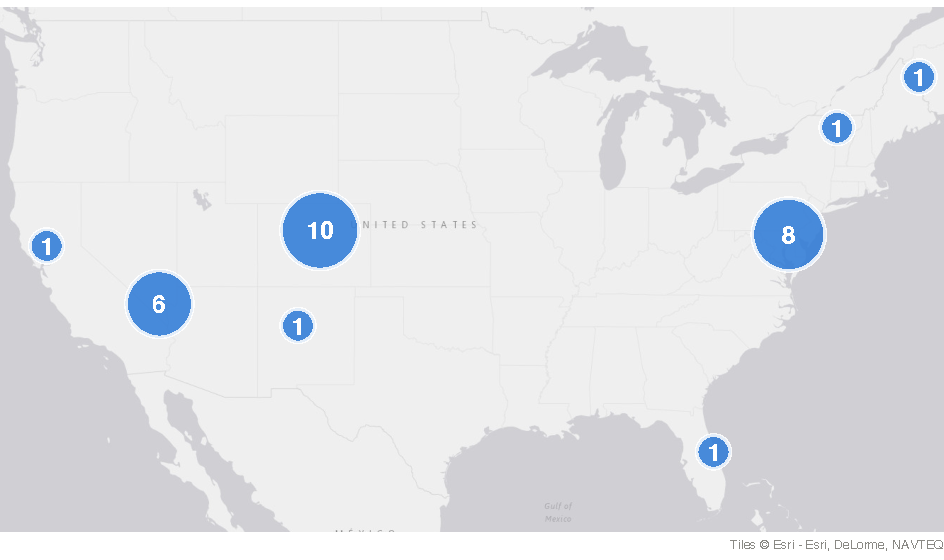
\includegraphics[width=\textwidth]{../methodsx_figures/out/fig_sites_map.pdf}
\caption{Locations of the \vNConfigured{} validation sites; numbers give the sites in each cluster. Station irradiance is from BMS for the \vNStationGolden{} Golden sites and from UNLV for the \vNStationLV{} southern Nevada sites. Coordinates and evidence class of every site are given in Table~\ref{tab:s_sites}. Basemap: Esri, DeLorme, NAVTEQ.}
\label{fig:sites_map}
\end{figure}

Each site was configured from its PVDAQ metadata alone: coordinates, altitude, orientation, module and inverter models and counts. Module parameters came from the CEC database entry of the recorded module at 22 sites and from the datasheet fit at 7, and $U_c$ from a sensor fit at \vUcFit{} site, the datasheet NOCT at \vUcNoct{} and the PVsyst mounting class at \vUcClass{} (Section~\ref{sec:thermal}). The age factor was $f_{\mathrm{deg}}=(1-0.005)^{a}$, with $a$ the system age in years at the middle of the scored year and 0.5\,\%/yr the median field degradation rate of Jordan and Kurtz~\cite{jordanKurtz2013degradation}. One year per site was scored, chosen from the measured series and irradiance coverage alone, and each run started at the beginning of that year with no snow cover and a clean array. These \vNInd{} sites form the independent validation set. At \vNCal{} further Mid-Atlantic sites, the measured output under modelled snow cover reached 0.64 to 0.76 of the snow-free output, so fast snow removal was set after comparison with model output; these calibrated sites are reported separately.

Extraction from the raw PVDAQ record and quality control used metadata, measured values and clear-sky irradiance; simulated output was not used. Clock offsets were corrected by the whole-hour shift that maximised the correlation with Ineichen clear-sky GHI~\cite{ineichenPerez2002}, and all labels were moved to UTC before hourly means were formed (Section~\ref{sec:s_qc}). All series of a site were scored on the same hours: daylight hours with clear-sky GHI above 50~W\,m$^{-2}$, outside outage days identified from the measured series, and with a value from every compared series. Fully snow-covered days are removed with the outage days, so the snow model is assessed on days with measurable output.

The validation assesses agreement between simulated and measured power at the one-hour implementation interval. It is not a forecast evaluation, because all inputs are contemporaneous historical observations or reanalysis estimates. Over the scored set $\mathcal{T}$ of $N$ hours, with simulated $P_s$ and measured $P_m$, the scores are
\begin{equation}
b=100\,\frac{\sum_{\mathcal{T}}(P_s-P_m)}{\sum_{\mathcal{T}}P_m},\qquad
\mathrm{NRMSE}=100\,\frac{\sqrt{N^{-1}\sum_{\mathcal{T}}(P_s-P_m)^2}}{N^{-1}\sum_{\mathcal{T}}P_m},
\label{eq:metrics}
\end{equation}
with the absolute bias $|b|$ and the Kling-Gupta efficiency (KGE) in its original form, with the ratio of standard deviations as variability term~\cite{guptaDecompositionMeanSquared2009}. The bias measures the error in total energy and the NRMSE the typical hourly error. Uncertainty within the scored year was estimated by a paired circular block bootstrap~\cite{kunschJackknifeBootstrapGeneral1989,politisRomano1992circular} over blocks of \vBlock{} consecutive retained days, wrapped at the end of the year, with \vReps{} replicates and a fixed seed; one series is closer to the measured output than another at a site when the 95\,\% interval of their paired difference excludes zero.

\subsection{Agreement with measured output}
\label{sec:performance}

\begin{table}[htbp]
\centering
\caption{Median scores against measured AC output across the \vNInd{} independent validation sites.}
\label{tab:val_summary}
\small
\begin{tabular}{l l r r r r}
\toprule
Series & Irradiance & $b$ (\%) & $|b|$ (\%) & NRMSE (\%) & KGE \\
\midrule
\RePV & ERA5 & \vMedSysEraBias & \vMedSysEraAbsBias & \vMedSysEraNrmse & \vMedSysEraKge \\
\RePV & NSRDB & \vMedSysNsrdbBias & \vMedSysNsrdbAbsBias & \vMedSysNsrdbNrmse & \vMedSysNsrdbKge \\
\addlinespace[2pt]
PVGIS & PVGIS-ERA5 & \vMedPvgisBias & \vMedPvgisAbsBias & \vMedPvgisNrmse & \vMedPvgisKge \\
\addlinespace[2pt]
Simple rating model & ERA5 & \vMedRatEraBias & \vMedRatEraAbsBias & \vMedRatEraNrmse & \vMedRatEraKge \\
Simple rating model & NSRDB & \vMedRatNsrdbBias & \vMedRatNsrdbAbsBias & \vMedRatNsrdbNrmse & \vMedRatNsrdbKge \\
\bottomrule
\end{tabular}
\end{table}

\begin{figure}[htbp]
\centering
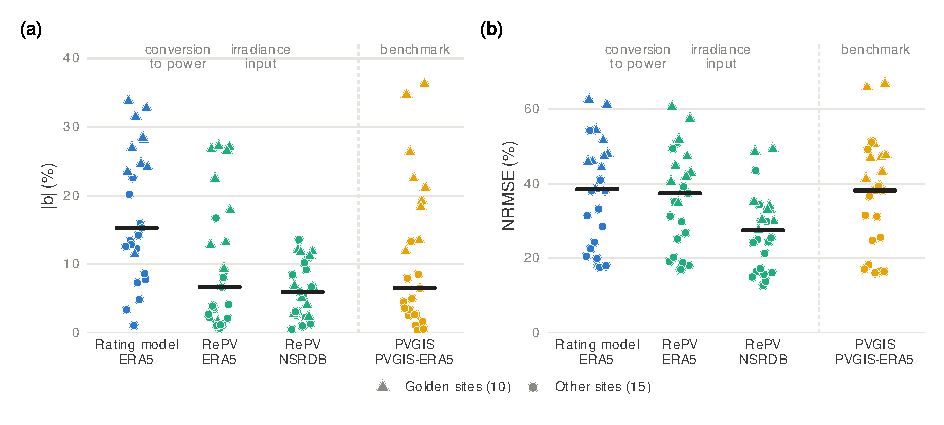
\includegraphics[width=\textwidth]{../methodsx_figures/out/fig_validation.pdf}
\caption{Absolute bias (a) and NRMSE (b) against measured AC output at the \vNInd{} independent validation sites. Each point is one site; triangles mark the \vNGolden{} Golden sites. From the simple rating model to \RePV{} on ERA5, only the conversion to power changes; from \RePV{} on ERA5 to \RePV{} on NSRDB, only the irradiance input changes. PVGIS-ERA5 is the independently developed reference model. Black bars are medians.}
\label{fig:validation}
\end{figure}

Table~\ref{tab:val_summary} gives the median scores and Figure~\ref{fig:validation} the scores of every independent site. On ERA5, \RePV{} reached a median absolute bias of \vMedSysEraAbsBias\,\% and an NRMSE of \vMedSysEraNrmse\,\%, against \vMedRatEraAbsBias{} and \vMedRatEraNrmse\,\% for the simple rating model: a large difference in total energy and a small one in hourly error. PVGIS-ERA5 reached \vMedPvgisAbsBias{} and \vMedPvgisNrmse\,\%; the paired intervals between \RePV{} on ERA5 and PVGIS-ERA5 included zero at \vPairEraPvgisAbsTie{} of the \vNInd{} sites for both $|b|$ and NRMSE, and PVGIS-ERA5 had the widest spread of all series, with biases from \vGoldenPvgisBiasLo{} to \vGoldenPvgisBiasHi\,\% at Golden.

The remaining ERA5 over-prediction was regional (triangles in Figure~\ref{fig:validation}a): at the \vNGolden{} Golden sites, the median bias was \vGoldenEraBiasMed\,\% on ERA5 and \vGoldenStnBiasMed\,\% on station irradiance. At the \vNCal{} calibrated sites, \RePV{} on NSRDB reached a median bias of \vCalSysNsrdbBias\,\% and an NRMSE of \vCalSysNsrdbNrmse\,\%.

\subsection{Irradiance input versus conversion to power}
\label{sec:sensitivity}

Exchanging one element at a time separated the effect of the irradiance input from that of the conversion to power (Figure~\ref{fig:validation}). Replacing ERA5 by NSRDB irradiance lowered the NRMSE of \RePV{} by a median of \vInputNrmseGain{} points per site (range \vInputNrmseGainLo{} to \vInputNrmseGainHi{}), with an interval excluding zero at all \vPairEraNsrdbN{} sites. Replacing the simple rating model with \RePV{} on ERA5 lowered it by \vPathRatNrmseGainEra{} points, and the input substitution produced the larger reduction at \vNInputBeatsPath{} of the \vNInd{} sites. At the \vNStation{} sites with station irradiance, the median NRMSE was \vStnSysEraNrmse, \vStnSysNsrdbNrmse{} and \vStnSysStnNrmse\,\% on ERA5, NSRDB and station irradiance, and the median bias \vStnSysEraBias, \vStnSysNsrdbBias{} and \vStnSysStnBias\,\%. \RePV{} on NSRDB had a lower NRMSE than PVGIS-ERA5 at \vPairPvgisNsrdbNrmseBetter{} of \vPairPvgisNsrdbN{} sites. In the evaluated data, the irradiance input therefore governed most of the hourly error, whereas the conversion to power mainly affected the error in total energy.

\subsection{Effect of individual components}
\label{sec:ablation}

Each component was removed from \RePV{} alone, with all others kept, and the change in signed bias $\Delta b$ was recorded (Table~\ref{tab:ablation}). The diffuse incidence-angle modifier changed the bias at every site, by a median of \vAblIamSysEra{} points on ERA5, and site-pressure air mass at most sites, most strongly at the high Golden and Albuquerque sites. The other components acted only where their triggering condition occurred: the complete snow treatment had the largest single effect, up to \vAblSnowSysEraLo{} points, and the 6~h snowfall trigger alone changed the bias at \vAblTrigSysEraAct{} sites, whereas placing losses before or after the inverter and the AC limit changed it only where the inverter or site limit was active. The terrain horizon changed no score, because the horizons reached at most \vHorizonMax$^{\circ}$. The snow-depth condition suppressed no snow event at the 17 sites with snowfall and reset the cover in at most 14 hours of a scored year, which changed the annual energy by at most 0.02\,\%, because ERA5-Land held at least 1~cm of snow whenever the trailing snowfall triggered an event and the arrays had shed their cover before the ground was bare. For these components, the evidence rests on the verification tests and the cited sub-models.

\begin{table}[htbp]
\centering
\caption{Change in signed bias $\Delta b$ (percentage points) when one component is removed from \RePV{}, across the \vNInd{} independent validation sites: median and range on ERA5, median on NSRDB, and number of sites where $|\Delta b|\geq0.1$ on ERA5. A positive $\Delta b$ means the component raises the simulated energy.}
\label{tab:ablation}
\small
\begin{tabular}{l r c r r}
\toprule
Component & ERA5 & range & NSRDB & sites \\
\midrule
\multicolumn{5}{l}{\emph{Active at all or most sites}} \\
Diffuse IAM & \vAblIamSysEra & \vAblIamSysEraLo{} to \vAblIamSysEraHi & \vAblIamSysNsrdb & \vAblIamSysEraAct/\vNInd \\
Site-pressure air mass & \vAblPresSysEra & \vAblPresSysEraLo{} to \vAblPresSysEraHi & \vAblPresSysNsrdb & \vAblPresSysEraAct/\vNInd \\
\addlinespace[3pt]
\multicolumn{5}{l}{\emph{Active where the triggering condition occurs}} \\
Complete snow model & \vAblSnowSysEra & \vAblSnowSysEraLo{} to \vAblSnowSysEraHi & \vAblSnowSysNsrdb & \vAblSnowSysEraAct/\vNInd \\
6~h snowfall trigger & \vAblTrigSysEra & \vAblTrigSysEraLo{} to \vAblTrigSysEraHi & \vAblTrigSysNsrdb & \vAblTrigSysEraAct/\vNInd \\
Snow-dependent albedo & \vAblAlbSysEra & \vAblAlbSysEraLo{} to \vAblAlbSysEraHi & \vAblAlbSysNsrdb & \vAblAlbSysEraAct/\vNInd \\
Physical loss placement & \vAblLossSysEra & \vAblLossSysEraLo{} to \vAblLossSysEraHi & \vAblLossSysNsrdb & \vAblLossSysEraAct/\vNInd \\
Soiling on irradiance & \vAblSoilSysEra & \vAblSoilSysEraLo{} to \vAblSoilSysEraHi & \vAblSoilSysNsrdb & \vAblSoilSysEraAct/\vNInd \\
AC capacity limit & \vAblClipSysEra & \vAblClipSysEraLo{} to \vAblClipSysEraHi & \vAblClipSysNsrdb & \vAblClipSysEraAct/\vNInd \\
\addlinespace[3pt]
\multicolumn{5}{l}{\emph{Triggering condition absent or rare in the validation data}} \\
Terrain horizon & \vAblHorSysEra & \vAblHorSysEraLo{} to \vAblHorSysEraHi & \vAblHorSysNsrdb & \vAblHorSysEraAct/\vNInd \\
Snow-depth condition and reset & \vAblDepthSysEra & \vAblDepthSysEraLo{} to \vAblDepthSysEraHi & \vAblDepthSysNsrdb & \vAblDepthSysEraAct/\vNInd \\
\bottomrule
\end{tabular}
\end{table}

%===========================================================================
\section{Limitations}
\label{sec:limitations}

\paragraph{Supported conditions.}
\label{sec:supported}
The validation covers monofacial fixed-tilt arrays from \vDcMin{} to \vDcMax~kWp, from sea level to \vAltMax~m, in desert, semi-arid, Mediterranean, humid subtropical and humid continental climates of the United States, at the one-hour implementation interval, with crystalline-silicon, CIS and CIGS modules. Tracker geometry, bifacial gain and the Sandia inverter model are implemented through pvlib sub-models but were not assessed empirically; the Sandia model was run only at the \vNSdm{} sites with a CEC inverter entry. At the one CIS site without a CEC entry, Golden~10, the datasheet fit kept the silicon band gap. Row effects and substantial terrain masking were not represented in the dataset, which had no recorded row layout and horizons of at most \vHorizonMax$^{\circ}$. Evidence for these components therefore rests on the verification tests and the cited sub-models.

\paragraph{System representation.}
Each run represents one array with a single orientation, module type and uniform electrical behaviour. Arrays with their own inverters can be run separately and their AC outputs summed. Arrays of different orientation on separate MPPT inputs of one inverter share its ceiling and part-load efficiency, which summing separate AC outputs does not reproduce. Parallel arrays on a single MPPT input operate at a common voltage that the method does not represent; they should be configured as one array of the dominant orientation, with the mismatch stated as an assumption. Availability and curtailment are applied outside the chain, and degradation enters as one constant factor per run, so a multi-year series carries the degradation of a single age unless the factor is updated per year.

\paragraph{Weather and metadata.}
Reanalysis and satellite irradiance carry spatial and temporal errors that propagate through every later stage; station irradiance reduces but does not remove them, because station-to-array distance, spatial mismatch and measurement error remain. Incomplete metadata transfers directly into output error: a surrogate module changes the low-light and temperature response, assumed geometry changes the diurnal and seasonal profile, and a misassigned mounting class biases summer output through the cell temperature.

\paragraph{Snow and soiling.}
The default soiling rate originates from California; elsewhere, regional deposition enters only through rainfall-driven cleaning frequency, and manual cleaning only through configured wash dates. Snow is removed by sliding, so melting on low-tilt arrays is delayed. Arrays cleared faster are represented by fast removal, a site property that the validation could identify only from measured output. The evidence for the 6~h trigger and the transmittance form of the snow loss is the annual bias at the snow-affected sites on days with measurable output; the snow cover itself was not observed, so this is evidence for the conversion chain on such days, not a validation of the cover state. Both states start from zero loss at the beginning of each run; a run whose first weeks fall in a snow season or a dry season should start some weeks earlier and discard that spin-up period.

\paragraph{Temporal and geographical transferability.}
The one-hour implementation does not resolve sub-hourly ramps or clipping within the hour. Each site contributed one year, so the scores describe agreement in the observed years, and the bootstrap intervals describe sampling within those years rather than interannual variability. All sites are from PVDAQ, and \vNGolden{} lie at Golden and \vNDesert{} in southern Nevada, so the cross-site medians weight these two regions most. Application beyond the assessed systems requires locally appropriate system metadata and parameters, in particular for snow, soiling and the mounting-dependent thermal behaviour.

%===========================================================================
\section*{Ethics statements}

The work used no human or animal subjects and no social media data. The measured PV data are the PVDAQ public datasets~\cite{deline2021pvdaq}, published under the Creative Commons Attribution licence.

\section*{CRediT author statement}

\textbf{Priyam Ketan Bhavsar:} Conceptualization, Methodology, Software, Validation, Formal analysis, Data curation, Writing (original draft), Visualization. \todo{Co-authors and roles.}

\section*{Acknowledgments}

\todo{Factor2 Energy GmbH, TUM chair, data providers (NREL PVDAQ and MIDC).}

This research did not receive any specific grant from funding agencies in the public, commercial, or not-for-profit sectors. \todo{Confirm.}

\section*{Declaration of interests}

The author declares no known competing financial interests or personal relationships that could have appeared to influence the work reported in this paper.

\section*{Supplementary material and/or additional information}

\paragraph{Supplementary material.}
The supplementary file contains the \RePV{} option specification (options of \RePV{} and of the simple rating model, weather field mapping, configuration groups and provenance classes, output series, module-parameter extraction, snow implementation details, worked example), the site data (selection, site list, surrogate modules, clock alignment), the data processing rules, the per-site scores with bootstrap intervals for every irradiance input and the computational performance. A repository supplement (\texttt{supplementary.md}) gives the verification tests with their acceptance criteria, the reproducibility settings, the pinned software environment and the ablations on every irradiance input.

\paragraph{Data availability.}
ERA5 and ERA5-Land data are available from the Copernicus Climate Data Store and through the Open-Meteo archive API; NSRDB irradiance from the NREL NSRDB API; MIDC station data from the NREL Measurement and Instrumentation Data Center; PVGIS horizons and reference series from the PVGIS API. Measured PV data are available from the PVDAQ public datasets~\cite{deline2021pvdaq} under the Creative Commons Attribution licence; the archived release redistributes the extracted hourly series of the assessment sites with attribution.

\paragraph{Code availability.}
Source code (Python package \texttt{solarmodel}, model \texttt{repv}), configuration schema, site files with provenance tables, example, verification suite, study files, pinned environment file and repository supplement, under the MIT licence: \url{https://github.com/princepriyam/RePV}, archived as \href{https://doi.org/10.5281/zenodo.24355624}{doi:10.5281/zenodo.24355624}.

\bibliographystyle{unsrtnat} % MethodsX: numbered Elsevier style (elsarticle-num) at submission
\bibliography{references}

\end{document}
